\section{Implementación}
\begin{frame}{Diagrama UML}
    \begin{figure}[H]
        \centering
        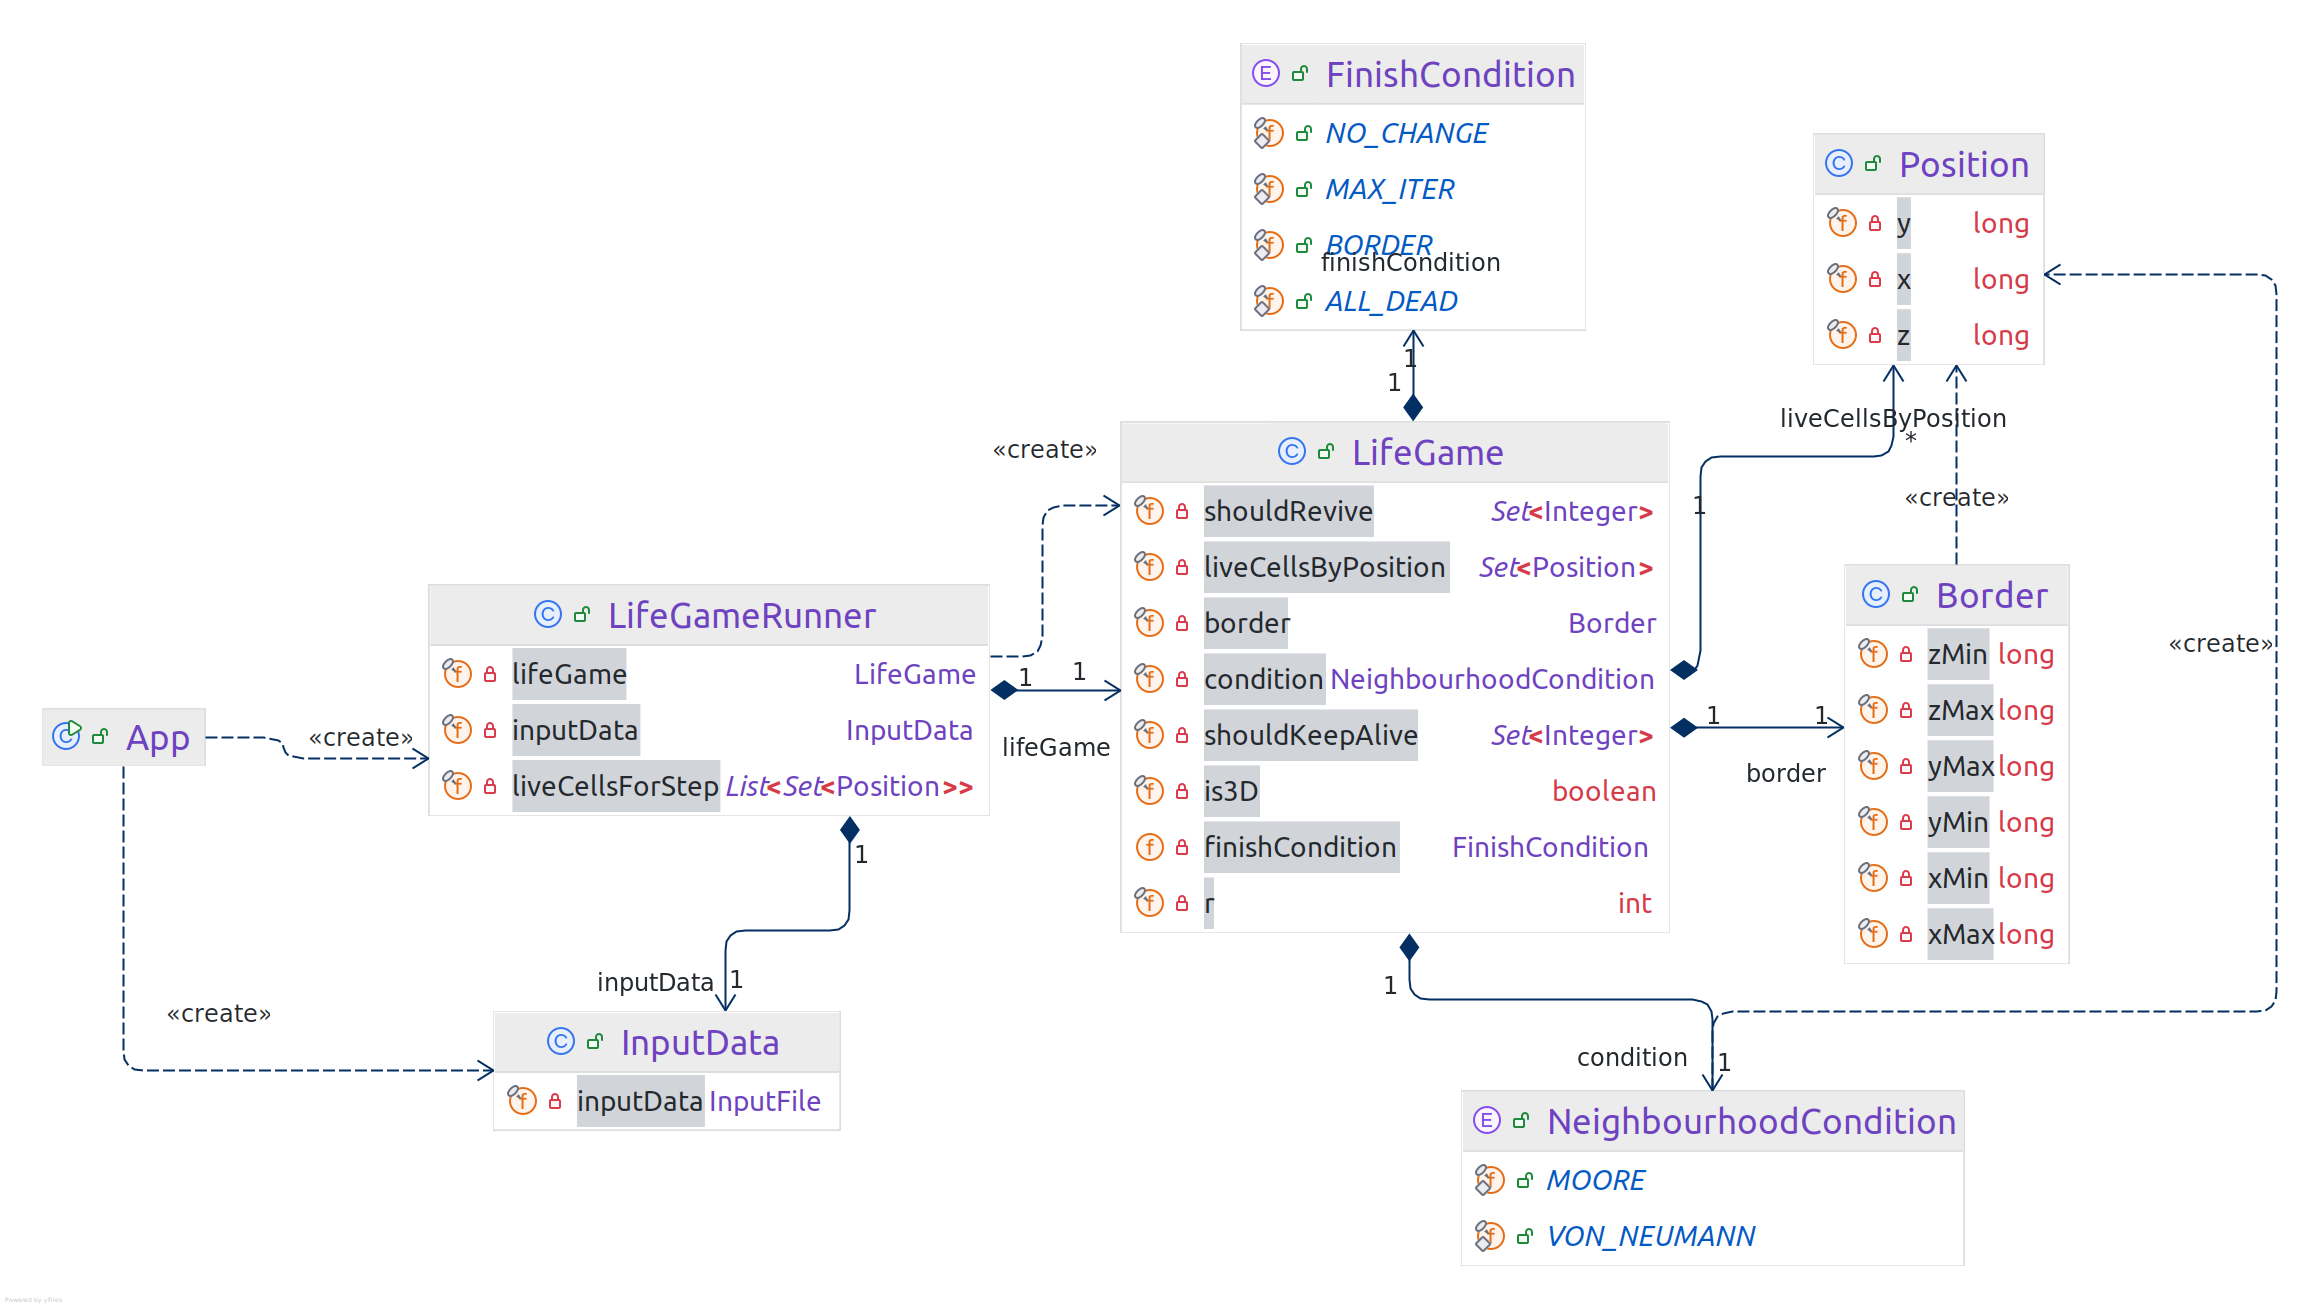
\includegraphics[width=0.9\linewidth]{pic/03-implementacion/UML}
    \end{figure}
\end{frame}

\begin{frame}{Motor de simulacion}


    \begin{minipage}[t]{0.55\linewidth}
        \begin{block}{Detalles de implementacion:}
            \begin{itemize}
                \item $GameOfLife$ y $GameOfLifeRunner$
                \item Matriz de celdas como una coleccion $SET$
                \item Condicion de corte:
                    \begin{itemize}
                        \item Borde
                        \item Ninguna viva
                        \item Limite de iteraciones
                        \item Sin cambio entre estados
                    \end{itemize}
                \item Código auxiliar: Borde, posicion y condicion de vecindario.
            \end{itemize}
        \end{block}
    \end{minipage}%
    \hfill%
    \begin{minipage}[t]{0.4\linewidth}
        \begin{figure}[H]
            \centering
            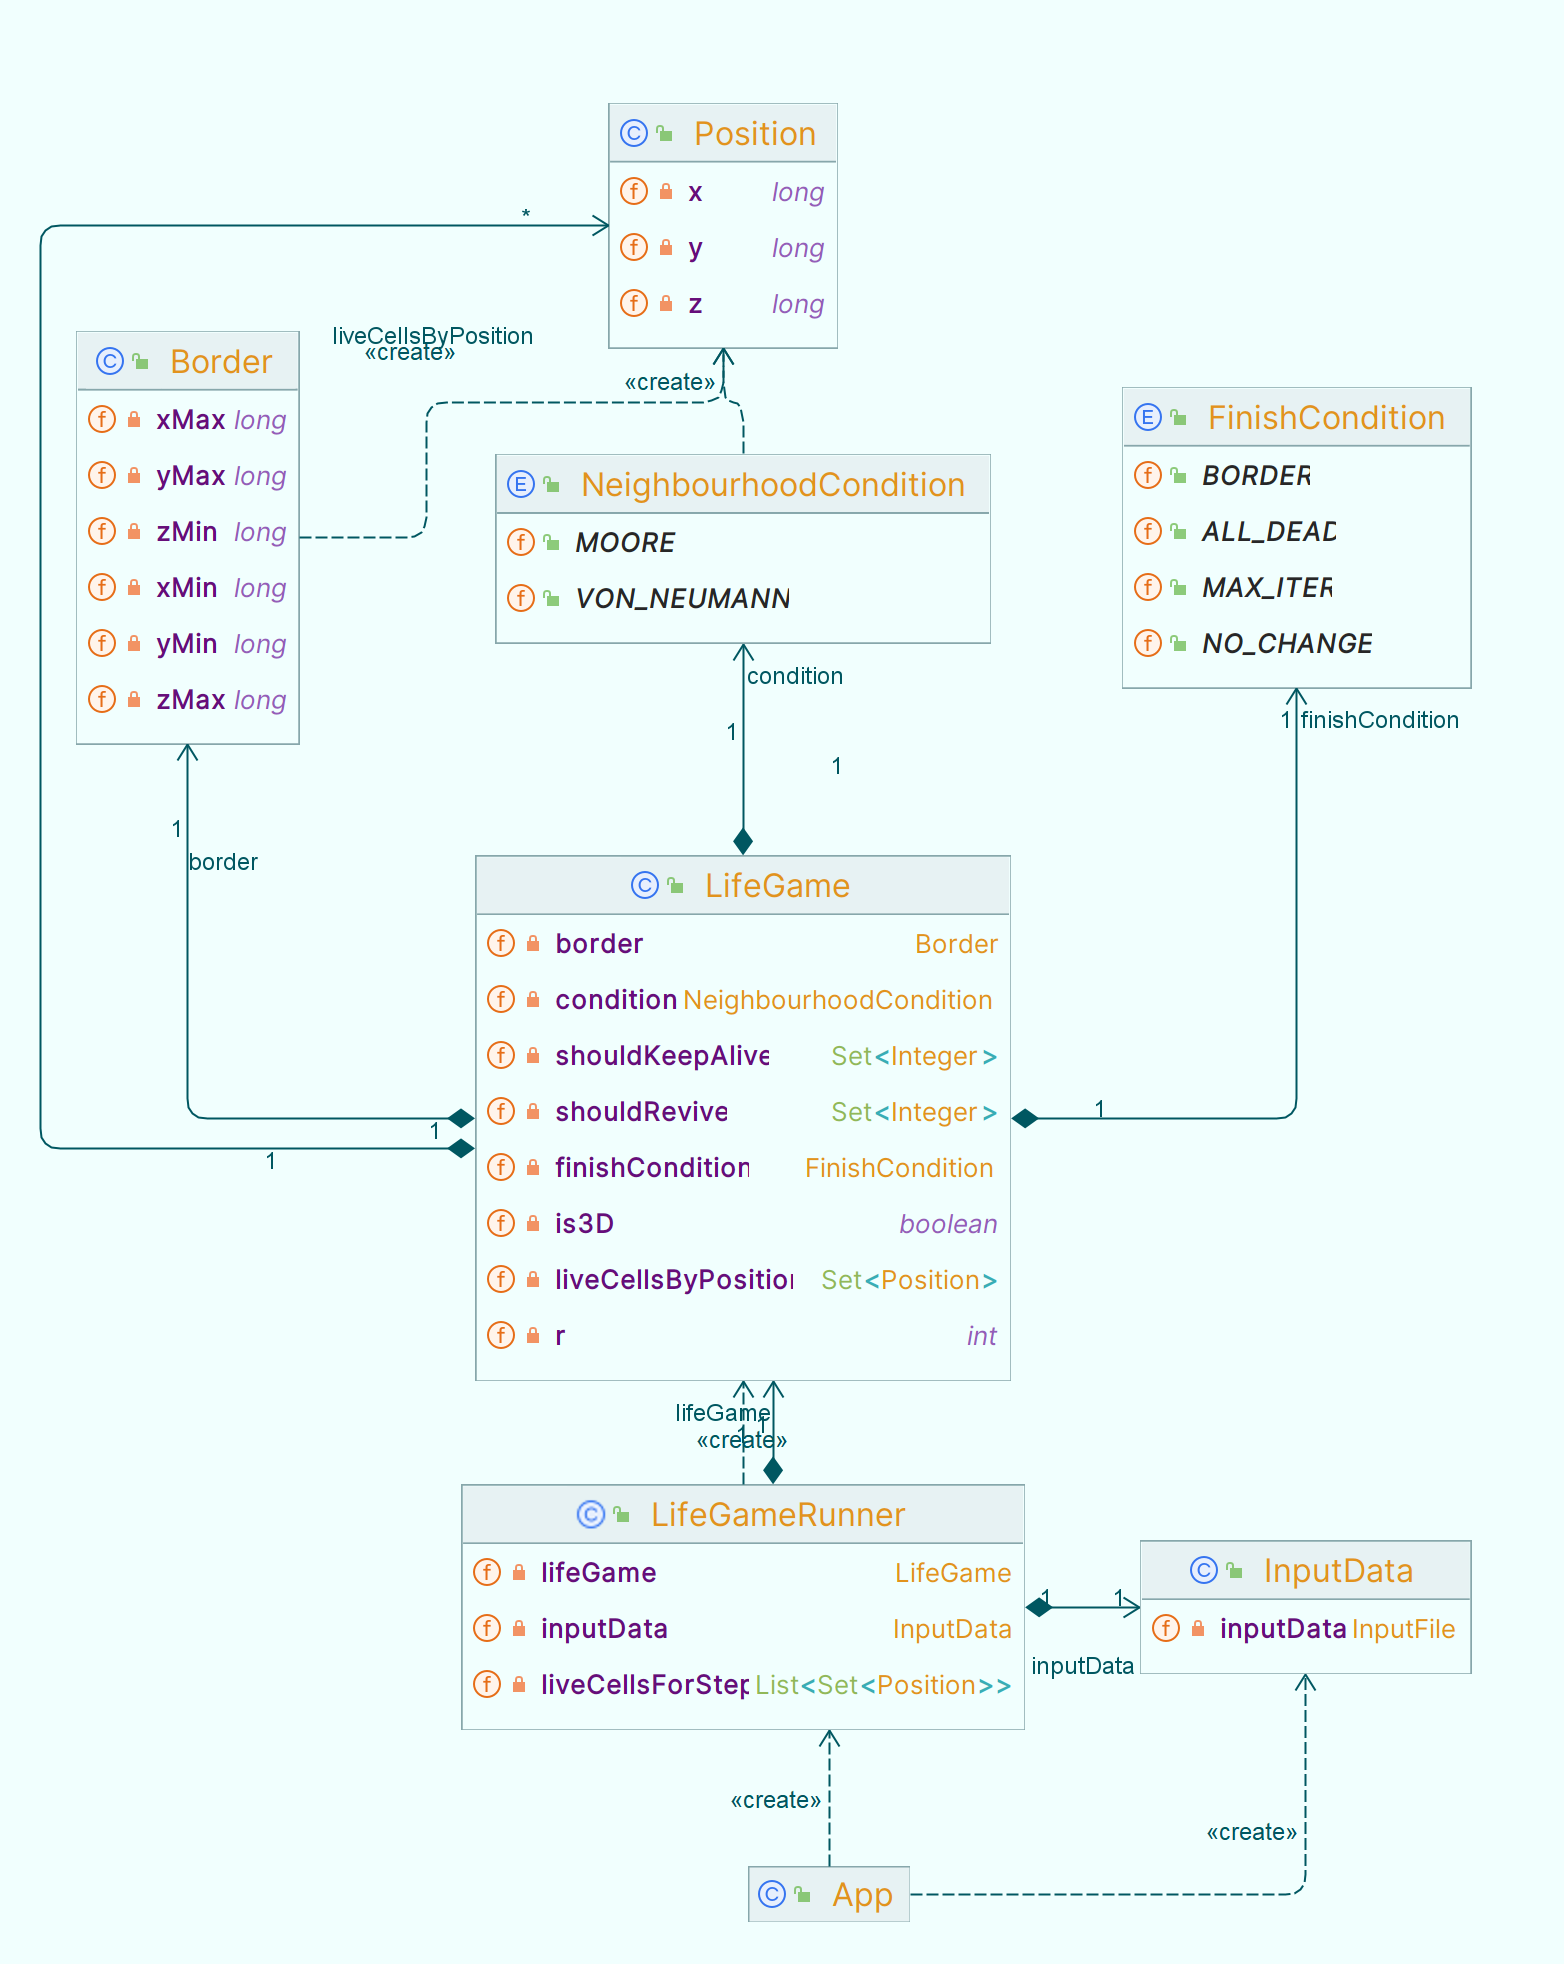
\includegraphics[width=0.9\linewidth]{pic/03-implementacion/UML_side}
        \end{figure}
    \end{minipage}
\end{frame}
